\documentclass{article}
\usepackage{hyperref}
\usepackage{amsmath}
\usepackage{amssymb}
\usepackage{pgfplots}
\usepackage{float}
\usepackage{todonotes}
\usepackage{tikz}

\renewcommand{\Re}{\mathbb{R}}
\newcommand{\Li}{\mathcal{L}}
\newcommand{\Ex}{\mathbb{E}}
\renewcommand{\Pr}{\mathbb{P}}
\newcommand{\Hy}{\mathcal{H}}

\newcommand\bigO[1]{
    \ensuremath{\mathcal{O}\left(#1\right)}
    }

\newcommand{\sigmoidPlot}{
    
    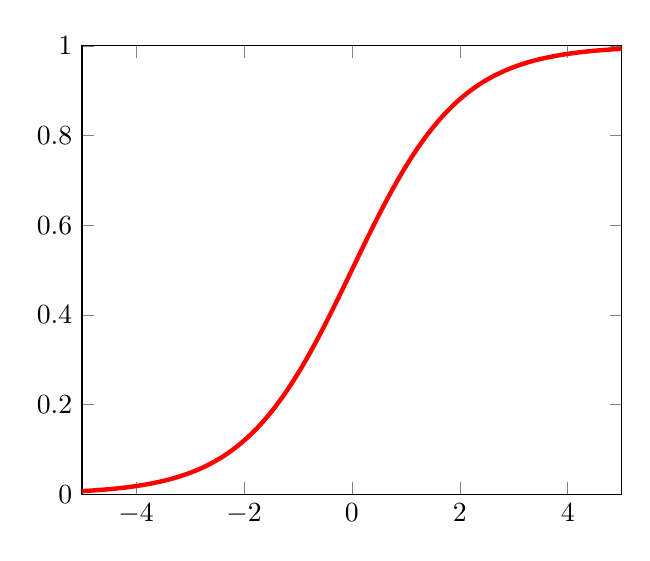
\begin{tikzpicture}
        \begin{axis}[xmin=-5, xmax=5, ymin=0, ymax=1, samples=150]
        \addplot[red, ultra thick] {1/(1+exp(-x))};
        \end{axis}
    \end{tikzpicture}
    
    }

\usetikzlibrary{positioning, calc}
\usetikzlibrary{arrows.meta}

\tikzstyle{circlebox}=[circle,thick,draw=black!75,minimum size=8mm]
\tikzstyle{inputnode}=[circlebox, draw=blue!75]
\tikzstyle{hiddennode}=[circlebox, draw=orange!75]
\tikzstyle{outputnode}=[circlebox, draw=orange!75]
\tikzstyle{simplebox}=[rectangle,thick,draw=black!75,
fill=black!20,minimum size=4mm]
\tikzstyle{textbox}=[rectangle,thick,minimum size=4mm,draw=black!0,
fill=black!0]
\tikzstyle{halfvdistance}=[yshift=-0.7cm]
\tikzstyle{abovebetween}=[xshift=-2.7mm]
\tikzstyle{edgepath} = [-Latex,->,shorten >=1pt,-stealth,semithick, rounded 
corners=5pt]

\def \nodedv {0.735cm}
\def \nodedh {0.65cm}

\tikzset{
    between/.style args={#1 and #2}{
        at = ($(#1)!0.5!(#2)$)
    }
}

\begin{document}
    \section{Subjects}
    \begin{itemize}
        \item What is protein tertiary structure?
        \item Computing a folding in the 2D HP model
    \end{itemize}
    
    \section{Notes}
    
    \subsection{Protein}
    Protein is made up of amino acids, which then folds into a 
    three-dimensional structure. Experiments show that they can unfold and 
    refold, which leads to the believe that the three-dimensional structure can 
    be found computationally from the information contained in the amino acid 
    sequence.
    
    The thermodynamical hypothesis states that the native structure of a 
    protein is the one for which the free energy is at a global minimum.
    
    If we were able to construct the tertiary structure from the primary 
    structure, we would be able to answer scientific questions like:
    \begin{itemize}
        \item What does the structure of protein $x$ look like?
        \item Can we predict the binding of of molecule $x$ to $y$?
        \item Does molecule $z$ has the potential to become a good drug 
        candidate?
        \item Can we find a promising subset of drug candidates from a huge 
        database containing millions of compounds?
    \end{itemize}
    
    A bit of background on genes, DNA etc. A cell has 46 chromosomes, DNA 
    molecules, which store genetic information. DNA's consist of nucleotides 
    (ACGT). Before a gene comes into use, its coding DNA is transcribed to RNA 
    which in turn is translated into a protein.
    
    An amino acid consists of a central carbon atom $C_\alpha$ which is bonded 
    to an amino group and a carboxyl group and a side-chain. The backbone in 
    proteins is the sequence of amino groups, $C_\alpha$ and carboxyl groups. A 
    gene reveals the blueprint of a protein, the structure is what we will try 
    to find.
    
    \begin{description}
        \item[Primary] the sequence of amino acids
        \item[Secondary] is either a $\alpha$-helix or a $\beta$-strand. They 
        are secondary structures that form while the protein is folded. This is 
        usually presented as a sequence of characters corresponding to the 
        individual amino-acids of e.g. $\alpha,\beta$.
        \item[Tertiary] the three-dimensional form the protein takes after 
        folding.
    \end{description}

    However, protein folding remains one fo the great unresolved problems of 
    molecular biology. So why do we even want to predict the protein 
    structures? Because X-Ray crystallography is expensive and time-consuming, 
    and some important proteins (membrane proteins) are difficult or impossible 
    to crystallize. Furthermore, doing simulations may provide us with new 
    knowledge about the physics, and help us understand mis-folding which 
    causes diseases.
    
    \subsection{HP Lattice models}
    In the HP-lattice models we want to predict protein structures by 
    minimizing free energy, under the assumption that formation of a 
    hydrophobic core is a primary force in protein structure formation.
    
    The HP-part is that we take the amino-acids and map them to either 
    hydrophilic (water loving) or hydrophobic (water hating) amino acids. This 
    isn't always so black and white, since some amino acids are not hydrophilic 
    or vice versa in all contexts.
    
    The lattice part is that we embed it into a lattice (i.e. a grid) and avoid 
    any overlaps. The aim is then to maximize the number of non-bonded H-H 
    contacts, and we just increment (or decrement for minimization) the score 
    by one for each pair of neighbouring non-diagonal, non-bonded lattice 
    points which are both H's.
    
    The result is that we the hydrophobic residues tend to be on the inside, 
    forming a hydrophobic core, and the hydrophilic residues on the outside.
    
    \begin{itemize}
        \item Residues are represented by a single atom, what about the 
        side-chains? Bonds are not mimicing 'reality'
        \item Electrostatic interactions (repulsion/attraction) are not 
        considered
        \item Energies are very short range
        \item Two residues must be an odd distance (of at least three) apart to 
        be in contact
        \item Does not reveal the structure of any particular protein
        \item For short sequences, all conformations can be found
        \item It's easy to understand for non-biologists and it is easy to 
        implement
    \end{itemize}
    The number of possible valid folds for a sequence of length $L$ on a 
    two-dimensional square lattice approaches $2.638^n$, so the number of 
    solutions is exponential in the length of the sequence being folded. 
    Finding an optimal solution is NP-complete!
    
    Various algorithms has been found:
    \begin{itemize}
        \item U-Fold: $\frac{1}{4}$ of the optimal
        \item S-Fold: Still $\frac{1}{4}$ of the optimal (though often better)
        \item C-Fold: Between $\frac{1}{4}$ and $\frac{1}{3}$ of the optimal
        \item Newman found a linear time $\frac{1}{3}$ approximatino
        \item There are numerous heuristics, like genetic, ant-systems etc.
    \end{itemize}
    
    U-Fold: 
    \begin{itemize}
        \item Mark every even $H$ with $e$ and every odd $H$ with $o$.
        \item Match even's from the left with odd's from the right (match 1). 
        Then odd's from the left with even's from the right (match 2). 
        \item Pick the biggest of match 1 and match 2
        \item Fold based on the match, such that every other grid point is 
        occupied by a matched $h$.
    \end{itemize}
    A $h$ can form at most $2$ bonds with $h$'s of opposite parity:
    \begin{equation*}
        OPT(S)\leq 2 \min(|Even(S)|,|Odd(S)|)
    \end{equation*}
    We then make a HP fold such that:
    \begin{align*}
        HP-Score(F) &\geq\text{ ``Size of matching''}\\
            &\geq \frac{1}{2}\min(|Even(S)|,|Odd(S)|)\\
            &\geq \frac{1}{2}(\frac{1}{2} OPT(S))\\
            &\geq \frac{1}{4} OPT(S)
    \end{align*}
\end{document}